% CUSTOM TEMPLATE FOR SOLUTIONS STARTS
\documentclass[answers]{exam}
 
 \usepackage{graphicx}
 \usepackage{float}
 \usepackage{amsmath}
 \usepackage{amsfonts}
 \usepackage{framed}
 \usepackage{algorithmicx}
 \usepackage{algpseudocode}
 \newcommand{\ans}[1]{\begin{framed}{\textbf{Answer:} #1}\end{framed}}
 \newcommand{\sol}{\uplevel{\textsc{Solution:}}}
 \newenvironment{answer}{%
     \renewcommand{\solutiontitle}{\noindent\textbf{Answer:}\enspace}
     \begin{solution}
     }{%
     \end{solution}
     \renewcommand{\solutiontitle}{\noindent\textbf{Solution:}\enspace}
 }
% CUSTOM TEMPLATE FOR SOLUTIONS ENDS

% First we setup the header and footer
\pagestyle{headandfoot}
\runningheadrule
\runningfootrule
\header{COL351: Analysis and Design of Algorithms (CSE, IITD, Semester-I-2020-21)}{}{Quiz 2}
\footer{}{\thepage  \, of \numpages}{}
 
% We want the points for each question displayed on the left
%\pointname{points}
%\pointsinmargin
 
% Automatically total the points - make sure to compile TWICE
\addpoints
 
\begin{document}


\vspace{0.1in}


\vspace{0.1in}
% Some general text together with number of questions and total points possible
There are \numquestions\, questions for a total of \numpoints\, points.
\vspace{0.1in}
\hrule
 \vspace{0.2in}
\begin{questions}
 
\question[3] 
Let us define the ``max-weight" of a spanning tree $T$ of a strongly connected, weighted, undirected graph $G$ to be the weight of the maximum weight edge in the spanning tree $T$. Also, let us define
    a ``minmax spanning tree" of a strongly connected, weighted, undirected graph $G$ to be a spanning tree with minimum value of max-weight.

(For example, consider a graph below on the left. The max-weight of the spanning tree in the middle is $5$. The minmax spanning tree of $G$ is shown on the right.)

    \begin{center}
        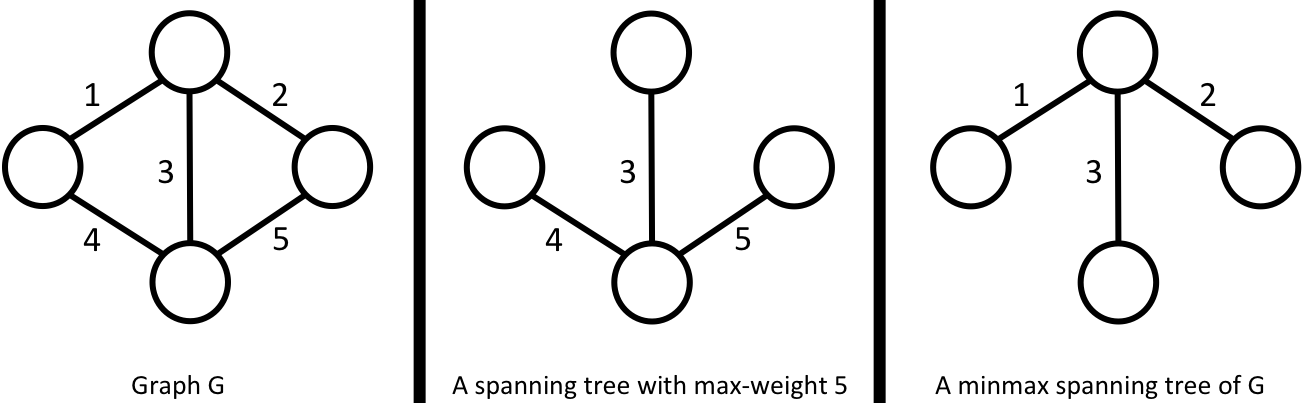
\includegraphics[scale=0.2]{img/minmax.png}
    \end{center}

Prove or disprove the following statement: 

    Let $G$ be any strongly connected, weighted, undirected graph. Any minimum spanning tree of $G$ is also a minmax spanning tree of $G$.

    \begin{solution}

        I will show that this property is true.

        Suppose that this is not true, and thus there exists a MST (say $T$) of $G$ which has an edge $e$ with higher weight than the edge $e'$ with the maximum weight in a minmax spanning tree (say
        $T'$) of G. We try adding $e$ to the tree $T'$. Since $T'$ is a tree, and $e$ is not in $T'$ (by weight of $e$), the addition induces a cycle. Hence, there is a cycle $C$ in the graph with the
        edge $e$, and all edges in the cycle have a weight $<$ weight of $e$.

        Now we claim that this leads to a contradiction.

        When we remove the edge $e$ from $T$, it breaks $T$ into two trees $T_1$ and $T_2$.

        Consider the set of vertices in the cycle $C$ in $T_1$ (say $S_1$) and the set of vertices in the cycle $C$ in $T_2$ (say $S_2$). Note that both of these are non-empty, since the endpoints of
        $e$ are not in the same tree.

        Then adding any edge of the cycle between one vertex in $S_1$ and another vertex in $S_2$ joins the trees $T_1$ and $T_2$ and is a spanning tree, with a weight strictly less than that of the
        spanning tree $T$, which is a contradiction since $T$ is, by definition, an MST of $G$.

        Hence, we have shown that our assumption was false, and thus any minimum spanning tree is also a minmax spanning tree of G.

    \end{solution}

\question[7]
        There are $n$ jobs that are supposed to be scheduled on a single machine. With each job $i$, there is an associated duration $t(i)$ that denotes the time that job $i$ will take to execute on
        the machine. Each job $i$ also has an associated weight $w(i)$ that denotes the importance of this job. Given a schedule, which is an ordering of jobs to be executed on the machine, the
        completion time of job $i$ is the time at which this job is finished by the machine. Let the completion time of job $i$ be denoted by $C(i)$. The cost $V$ of a schedule is defined as $V =
        \sum_{i=1}^{n} w(i) \cdot C(i)$. You are supposed to design an algorithm for giving a schedule with minimum cost.

        (For example, consider three jobs with their duration and weight given in the table below. If the schedule is $(1, 2, 3)$, then $C(1) = 2, C(2) = 6$, and $C(3) = 9$. So, the cost of this
        schedule is $2 \cdot 3 + 1 \cdot 6 + 2 \cdot 9 = 30$.)

        \begin{center}
        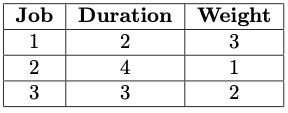
\includegraphics{img/table.png}
        \end{center}

Answer the following:

\begin{parts}

    \part Give the schedule for the above example that has the minimum cost.

    \begin{answer}
        Order of job numbers: $1, 3, 2$, cost = $25$. 

        These jobs should be completed one after the other without any time gap.
    \end{answer}

    \part  Consider the following greedy strategy for this problem:

    Trial greedy strategy: Do the jobs in increasing order of duration (breaking ties arbitrarily).

Show that this strategy does not always outputs a schedule with minimum cost.

    \begin{answer}
        Consider the following set of jobs:

        \begin{center}
        \begin{tabular}{|c|c|c|}
            \hline
            Job & Duration & Weight\\
            \hline
            1   &    2     &      1\\
            \hline
            2   &    3     &      2\\
            \hline
            3   &    4     &      3\\
            \hline
        \end{tabular}
        \end{center}

If we do them in the increasing order of duration, we get a cost of 39. However, if we do them in the reverse order, we get a cost of 35, which is strictly less than 39, and thus the greedy algorithm doesn't always output a schedule with minimum cost since there is a schedule with a smaller cost.
    \end{answer}

    \part Design a greedy algorithm for this problem. Give proof of correctness using "modify-the-solution" method. Give a running time analysis of your algorithm.

    \begin{answer}

        \textbf{Greedy strategy:}
        Among all remaining jobs, run the job with the least value of $d(i)/w(i)$, and recursively run the remaining jobs with the same strategy.

        \textbf{Proof of correctness:}

        Exchange lemma: Given any solution $OS$, we can construct a solution $OS'$ whose first decision is given by the greedy strategy and it is at least as good as $OS$.

Consider any solution $OS$. We will construct a solution $OS'$ with the first decision matching the greedy decision.

Suppose the job with least $d/w$ is at index $i$ in the solution $OS$, and let the corresponding duration and weight be $d, w$ respectively. Let the job at the first index in $OS$ have duration and
        weight $d', w'$ respectively.

        Let $OS = o_1, o_2, ..., o_n$. Then $OS' = o_i, o_1, ..., o_{i - 1}, o_{i + 1}, ..., o_n$. This is valid since we consider all jobs in non-overlapping fashion and because of validity of $OS$.

Let $d_i$ = duration of job $i$ and let $w_i$ be the weight of job $i$ and let $a_i$ = $d_i/w_i$.

        Then $V(OS') - V(OS)$ is (upon simplification) $w_1 w_i (a_i - a_1) + w_2 w_i (a_i - a_2) + \ldots + w_{i - 1} w_i (a_i - a_{i - 1})$. Since $a_i \le a_r$ for all $r$, we have that $V(OS) \ge
        V(OS')$, and our exchange lemma is proved.

Now we prove by induction the fact that for any problem the greedy strategy gives the optimal solution

Base case: For a problem with no jobs, we are trivially done.

Induction step: Let $P$ be an instance of a problem with $n$ elements.
Let $GS(P)$ be the greedy solution for $P$, and $OS(P)$ be any solution. Define $OS'$ as in the exchange lemma (valid since we schedule all jobs) and let $OS'$ = first job + $OS''$ and $GS(P)$ = first
        job + $GS'$. Then we have

$V(GS(P))$ = cost of first element $\times$ sum of weights + $V(GS') \le$ cost of first element $\times$ sum of weights + $V(OS'') = V(OS') \le V(OS)$,
where the first inequality comes from the induction hypothesis.

        \textbf{Algorithm:}

        \begin{algorithmic}
            \Function{Solve}{$d[1..n], w[1..n]$}
                \State let $a$ be the identity permutation on $[1..n]$.
                \State sort $a$ in non-decreasing order of $d/w$.
                \State \Return $a$
            \EndFunction
        \end{algorithmic}

        \textbf{Runtime analysis:}

        Sorting takes $O(n \log n)$ time where $n$ is the number of jobs, and returning takes $O(n)$ time, so the whole algorithm takes $O(n \log n)$ time.
    \end{answer}

\end{parts}

\end{questions}
\end{document}

